% !TeX program = xelatex
% 完整中文审读稿；与英文稿保持相同内容、公式和结果。
\providecommand{\PaperRoot}{./}
\makeatletter\edef\input@path{{\PaperRoot}{\PaperRoot template/}}\makeatother
\PassOptionsToPackage{no-math}{fontspec}
\documentclass[a4paper,fleqn]{cas-sc}
\usepackage[UTF8,scheme=plain,fontset=windows]{ctex}
\usepackage[numbers,sort&compress]{natbib}
\usepackage{bm,tabularx,algorithm,algpseudocode,placeins}
\graphicspath{{\PaperRoot}}
\renewcommand{\figurename}{图}
\renewcommand{\tablename}{表}
\renewcommand{\refname}{参考文献}
\floatname{algorithm}{算法}
\algrenewcommand{\algorithmicrequire}{\textbf{输入：}}
\newcommand{\R}{\mathbb R}
\newcommand{\C}{\mathbb C}
\newcommand{\E}{\mathbb E}
\newcommand{\Rea}{\operatorname{Re}}
\newcommand{\tr}{\operatorname{tr}}
\begin{document}
\let\WriteBookmarks\relax
\shorttitle{未知宽带强弱重叠源的高效直接定位}
\shortauthors{B. Hao et al.}
\title[mode=title]{未知宽带强弱重叠源的高效直接定位：多候选联合精修与波形消元更新}
\author[inst1]{Benjian Hao}[orcid=0000-0002-6676-7306]
\ead{bjhao@xidian.edu.cn}
% TODO(CRediT): Add approved roles after all authors confirm them.
\author[inst1]{Xinlei Wang}[orcid=0000-0002-6855-3686]
\ead{wangxinlei@stu.xidian.edu.cn}
% TODO(CRediT): Add approved roles after all authors confirm them.
\author[inst1]{Zan Li}[orcid=0000-0002-5207-6504]
\cormark[1]
\ead{zanli@xidian.edu.cn}
% TODO(CRediT): Add approved roles after all authors confirm them.
\cortext[cor1]{Corresponding author.}
\affiliation[inst1]{organization={State Key Laboratory of Integrated Service Networks, School of Telecommunications Engineering, Xidian University},
  city={Xi'an}, postcode={710071}, country={China}}
\begin{abstract}[摘要]
频谱重叠与接收功率不均衡增加了两步定位中逐源时延提取和关联的难度。直接位置估计联合拟合多站混合观测，其高效求解仍需选择候选区域，并精修与未知波形耦合的位置参数。本文在已知相对幅度与基带时延模型下，针对同步单天线站的这两个求解环节提出改进。多候选联合精修交替投影（MCJ-AP）保留分离的条件谱峰，在联合调整两源位置后选择分支；波形消元块Newton正交匹配追踪（VP-BNOMP）将当前源波形的消元纳入局部位置曲率。20个源位置构型的2400条观测中，五候选将双源20\,m成功率由95\%提高至99\%；额外恢复来自一个构型，且大多需要第五候选。在相同候选及共同投影梯度停止容差下，联合精修减少31.36\%的平均完整耗时。另一组240条配对观测在相同消元接受目标下，分离出消元曲率带来的83.77\%平均降时。新源位置测试进一步显示了额外AP候选只增加成本而不增加恢复、以及VP仍有定位失败的情况。实验量化了候选保留的恢复--成本权衡，以及波形消元曲率的局部计算收益。
\end{abstract}
\begin{keywords}[关键词]
直接位置估计\sep 重叠源\sep 交替投影\sep 块NOMP\sep 变量投影
\end{keywords}
\maketitle

\FloatBarrier
\section{引言}
辐射源定位常先估计到达时间差，再求解位置。广义互相关与双曲线定位为这一两步流程提供了成熟工具\cite{KnappCarter1976,ChanHo1994}。未知源占用相同频带时，各站收到的是不同传播响应下的混合信号，逐源时延的提取与关联随之变难，强源存在时的弱源尤其如此。直接位置估计（DPD）将传播关系纳入观测模型，联合利用多站数据估计位置\cite{ChenHudsonYao2002,WeissAmar2005}。

本文研究四个同步单天线站观测两个独立未知宽带源的场景。源位置、发射波形与功率未知，站点坐标及相对传播响应已知。单源谱中的多个高峰可能都由强源形成，而同时穷举两个二维位置需要检查大量组合。逐源发现与连续精修可以减少搜索量，剩余困难出现在不同环节：过早舍弃候选可能丢失有效的精修分支，位置与未知波形的耦合则可能增加局部更新成本。

宽带最大似然与交替投影（AP）通过固定其他位置、更新当前源来降低联合搜索维数\cite{ChenHudsonYao2002}。MUSIC型DPD利用候选响应与估计噪声子空间的正交关系\cite{WeissAmar2005}；MVDR利用协方差逆矩阵抑制干扰\cite{Capon1969}，DPD-HR将其用于直接定位\cite{TirerWeiss2016}。这些方法处理混合信号的方式不同，表现也受协方差估计与搜索影响。因此，本文在相同数据和传播信息下比较具体实现。

Newton正交匹配追踪（NOMP）结合贪心发现、Newton精修和循环更新\cite{Mamandipoor2016}。Yang等的二维多频块NOMP将同一位置的逐频未知系数组成一块，在位置更新后重估系数\cite{Yang2022}，是本文局部更新的直接参照。QNOMP从导频信道观测中消去路径增益，联合精修时延与角度\cite{Zeng2025}。本文的未知量则是各源在每个保留频点的波形系数，非线性参数为源位置。

候选选择也有相关研究。Oh与Un先通过顺序MUSIC形成初值，再执行AP更新\cite{OhUn1991}；LAOLS补全临时支持集后，用残差比较离散原子候选\cite{Chatterjee2012}。MCJ-AP按条件投影评分保留分离的空间峰，再对每个分支连续精修两源位置。条件评分已消去两源波形，但固定了第一源位置；联合拟合还允许该位置移动，因此初始排名较低的条件峰可能得到更好的联合定位解。MCJ-AP据此将分支选择推迟到连续拟合之后，无需为每个分支重复全域扫描。

未知波形的处理还影响精修成本。变量投影先消去线性系数，再优化非线性参数\cite{GolubPereyra1973}。本文将所得可按频率分解的曲率纳入块NOMP局部位置更新，并在相同接受目标下与固定系数曲率比较。两种方法在同一宽带定位模型下分别处理候选选择和局部更新成本，是独立的求解方案。本文的贡献为：
\begin{enumerate}
\item MCJ-AP将分支选择推迟到连续联合拟合之后。保存分支分析识别低排名条件峰带来的恢复；同候选配对比较则将覆盖收益与联合精修相对交替精修的计算节省分开。
\item VP-BNOMP在保留残差发现和循环块更新的同时，采用波形消元后的位置曲率。逐频小矩阵构造与局部曲率分析解释其更新机制，相同接受目标下的比较分离出精修成本收益，并与完整定位可靠性区分。
\end{enumerate}
实验在共同240条观测上比较八类方法，在2400条观测上评价主要方法，并以新源位置的480条观测检验冻结配置。各批次的接收站坐标不变，分别考察候选恢复与局部计算收益。

\FloatBarrier
\section{观测模型与定位目标}
\FloatBarrier
\subsection{同步宽带观测}
设第$l$个站的位置为$\bm r_l\in\R^2$，$l=1,\ldots,L$；第$k$个源的位置为$\bm p_k\in\Omega\subset\R^2$，$k=1,\ldots,K$。假设静态直达传播，站间时间与频率同步，接收链路相对响应已标定，天线极化匹配且方向响应一致。实验采用$L=4$和已知$K=2$。定义
\begin{equation}
d_{lk}=\|\bm p_k-\bm r_l\|_2,\qquad
\tau_{lk}=d_{lk}/c_0,\qquad \beta_{lk}=d_{lk}^{-1},
\label{en:distance}
\end{equation}
其中$c_0$为传播速度。远场、极化匹配的理想各向同性天线满足自由空间衰减关系
\begin{equation}
P_{\rm r}/P_{\rm t}=(\lambda/4\pi d)^2,\qquad
a_{\rm amp}(d)=\sqrt{P_{\rm r}/P_{\rm t}}=\lambda/(4\pi d).
\label{en:freespace}
\end{equation}
其中$P_{\rm r}$、$P_{\rm t}$分别为接收与发射功率，$\lambda$为波长\cite{ITURP5252024}。波长与天线响应固定时，公共因子$\lambda/(4\pi)$可并入未知波形，站间相对幅度因此与$1/d$成正比。

传播相位采用理想基带纯时延模型。链路标定消除站端响应，基带纯时延则是另外规定的传播假设。生成器与定位器使用同一基带模型，不引入射频载波相位或随机链路增益。采样率为$f_s$、记录为$N$点时，
\begin{equation}
x_l[n]=\sum_{k=1}^K\beta_{lk}s_k(n/f_s-\tau_{lk})+w_l[n],
\quad 0\le n<N,
\end{equation}
其中$s_k$包含未知发射功率与公共幅度因子，各源波形独立。噪声在站间和采样点间独立，与信号独立，服从$\mathcal{CN}(0,\sigma_t^2)$。

离散傅里叶变换（DFT）为
\begin{equation}
X_l(f_m)=N^{-1}\sum_{n=0}^{N-1}x_l[n]e^{-\mathrm j2\pi mn/N},
\qquad f_m=mf_s/N,
\label{en:dft}
\end{equation}
其中$m$为有符号频率索引。保留公共频带$\mathcal F$内的$F=|\mathcal F|$个频点，得到
\begin{align}
\bm x_f&=\bm A_f(\bm P)\bm s_f+\bm n_f,\label{en:frequency}\\
[\bm a_f(\bm p)]_l&=d_l(\bm p)^{-1}
 \exp[-\mathrm j2\pi f d_l(\bm p)/c_0],\label{en:response}\\
\bm A_f(\bm P)&=[\bm a_f(\bm p_1),\ldots,\bm a_f(\bm p_K)].\nonumber
\end{align}
这里$\bm x_f,\bm n_f\in\C^L$，$\bm s_f\in\C^K$，$\bm P=[\bm p_1,\ldots,\bm p_K]\in\R^{2\times K}$。$f$为有符号基带频率，$\mathrm j^2=-1$。共同窗近似忽略各站记录边缘的差异\cite{ChenHudsonYao2002}，其影响在第\ref{en:windowcheck}节核验。选频不改变噪声方差$\sigma_f^2=\sigma_t^2/N$或DFT归一化。

计算中可采用单位范数响应$\bm q_f=\bm a_f/\|\bm a_f\|_2$。同一响应列的公共缩放可由自由系数吸收，不改变站间相对幅度。实现对小于1\,m的距离作保护，所有仿真源均远离该区域。上标$H$、$T$和$\dagger$分别表示共轭转置、转置与伪逆。

记$P_{lk}$为源$k$单独在站$l$产生的时间平均接收功率，$B$为名义信号带宽。定义
\begin{equation}
\mathrm{SNR}_{k,\mathrm{in}}=10\log_{10}
 \frac{L^{-1}\sum_lP_{lk}}{\sigma_t^2 B/f_s},\qquad
\Delta=10\log_{10}\frac{\sum_lP_{l1}}{\sum_lP_{l2}}.
\label{en:snr}
\end{equation}
缩放源1时，源2与噪声保持不变，因此改变$\Delta$不改变弱源SNR。$\Delta>0$时称两源为强源和弱源；$\Delta=0$时仍保留A、B身份。单个站的局部功率差不必等于$\Delta$。

\FloatBarrier
\subsection{未知波形消元}
将逐频系数视为确定性未知量。在独立、等方差复高斯噪声模型下，最大似然等价于最小二乘。以观测能量$E_x=\sum_f\|\bm x_f\|^2>0$归一化，定义
\begin{align}
\mathcal L(\bm P,\{\bm s_f\})&=E_x^{-1}\sum_f
 \|\bm x_f-\bm A_f(\bm P)\bm s_f\|^2,\\
\widehat{\bm s}_f(\bm P)&=\bm A_f(\bm P)^\dagger\bm x_f,\label{en:waveLS}\\
J(\bm P)&=E_x^{-1}\sum_f\|\bm\Pi_{\bm A_f}^{\perp}\bm x_f\|^2,
\quad \bm\Pi_{\bm A_f}^{\perp}=\bm I-\bm A_f\bm A_f^\dagger.
\label{en:profile}
\end{align}
代入最小二乘波形后得到仅含位置的目标$J$\cite{GolubPereyra1973}，表示位置集合无法解释的观测能量比例。双源定位只含四个实位置变量，每次试探均重估系数。单源评分为
\begin{equation}
Q_0(\bm p)=E_x^{-1}\sum_f
 \frac{|\bm a_f(\bm p)^H\bm x_f|^2}{\|\bm a_f(\bm p)\|^2}.
\label{en:single}
\end{equation}
单源时$J=1-Q_0$。从$Q_0$中取两个峰没有共同拟合两个源；后续算法通过多源目标处理源间影响。

\FloatBarrier
\section{候选保留与波形消元精修}
\FloatBarrier
\subsection{条件搜索与MCJ-AP}
以$\bm B_f$表示已选位置的响应，对数据和试探响应作相同投影：
\begin{equation}
\bm r_f=\bm\Pi_{\bm B_f}^{\perp}\bm x_f,\qquad
\bm u_f(\bm p)=\bm\Pi_{\bm B_f}^{\perp}\bm a_f(\bm p).
\end{equation}
AP条件评分为
\begin{equation}
Q_{\rm AP}(\bm p\mid\bm B)=E_x^{-1}\sum_f
 \frac{|\bm u_f(\bm p)^H\bm r_f|^2}{\|\bm u_f(\bm p)\|^2}.
\label{en:conditional}
\end{equation}
当$\bm u_f\ne0$时，正交投影满足
\begin{equation}
\bm\Pi_{[\bm B_f,\bm a_f]}^{\perp}
=\bm\Pi_{\bm B_f}^{\perp}-\frac{\bm u_f\bm u_f^H}{\|\bm u_f\|^2},
\qquad J_{\rm B}-J([\bm B,\bm a(\bm p)])=Q_{\rm AP},
\label{en:gain}
\end{equation}
其中$J_{\rm B}=E_x^{-1}\sum_f\|\bm r_f\|^2$。固定已有位置时，最高条件评分对应最大的联合残差下降\cite{ChenHudsonYao2002}。计算采用归一化响应列；投影后范数平方不超过$10^{-20}$的频点评分置零，SVD伪逆的相对截断阈值为$10^{-10}$。投影恒等式适用于不受这些数值秩截断影响的区域。

MCJ-AP先在公共网格$\mathcal G$上最大化$Q_0$，连续精修第一源至$\bm p_1^{(0)}$。固定该位置后，扫描$Q_{\rm AP}$并保留间隔至少为$\Delta_c$的$M$个局部极大值$\bm c_m$，分别构成联合初值：
\begin{equation}
\widehat{\bm P}^{(m)}=\operatorname{LocalMin}_{\bm P\in\Omega^2}
 J(\bm P;[\bm p_1^{(0)},\bm c_m]),\qquad
m^*=\arg\min_m J(\widehat{\bm P}^{(m)}).
\label{en:branch}
\end{equation}
输出为$\widehat{\bm P}^{(m^*)}$。条件评分在第一源位置固定时排列候选，联合精修则移动两个位置并重估两源波形。因此，MCJ-AP在网格阶段保留候选集合，最终按精修后的$J$选择分支。若已有分支的解保持不变，扩大的嵌套集合不会增加所选残差。这一性质针对拟合目标，定位误差另行评价。

联合精修采用有界L-BFGS-B\cite{Byrd1995}。令$\bm\theta=\operatorname{vec}(\bm P)$，$\bm e_f=\bm x_f-\bm A_f\widehat{\bm s}_f$。当$\bm A_f$局部满列秩时，$\bm A_f^H\bm e_f=0$使系数导数项消失，得到
\begin{equation}
\frac{\partial J}{\partial\theta_i}=-\frac{2}{E_x}\Rea\sum_f
 \bm e_f^H\frac{\partial\bm A_f}{\partial\theta_i}\widehat{\bm s}_f.
\label{en:gradient}
\end{equation}
令$\bm v_l=(\bm p-\bm r_l)/d_l$，响应导数为
\begin{equation}
\nabla_{\bm p}a_l(f,\bm p)=a_l(f,\bm p)
 (-d_l^{-1}-\mathrm j2\pi f/c_0)\bm v_l.
\end{equation}
两项分别来自幅度与时延变化。联合Hessian由$2\times2$块$H_{ij}=\partial^2J/(\partial\bm p_i\partial\bm p_j^T)$组成：
\begin{equation}
H_{\rm joint}=\begin{bmatrix}H_{11}&H_{12}\\H_{21}&H_{22}\end{bmatrix}.
\end{equation}
L-BFGS-B由位置与梯度差近似联合曲率，不显式计算源间交叉块。同时更新两源位置可能减少反复条件拟合；第\ref{en:refinementcost}节在相同候选下评价这一成本，与候选恢复收益分开。

\begin{algorithm}[H]
\caption{MCJ-AP}\label{en:algap}
\begin{algorithmic}[1]
\Require 观测、站点坐标、网格$\mathcal G$、候选数$M$
\State 最大化$Q_0$，连续精修第一源位置
\State 固定该位置，扫描$Q_{\rm AP}$
\State 按评分降序保留$M$个满足间隔要求的局部极大值
\For{每个保留候选}
\State 从相应位置对联合最小化$J$，每次试探重新拟合全部系数
\EndFor
\State 输出最终$J$最小的分支
\end{algorithmic}
\end{algorithm}

\FloatBarrier
\subsection{波形消元块NOMP}
VP-BNOMP保留残差发现与循环位置更新\cite{Mamandipoor2016,Yang2022}。更新源$j$时，固定其他源已拟合的贡献：
\begin{equation}
\bm y_{j,f}=\bm x_f-\sum_{k\ne j}\bm a_f(\bm p_k)\widehat s_{k,f}.
\end{equation}
对试探位置$\bm p$，消去当前源系数：
\begin{align}
\widehat q_f(\bm p)&=\frac{\bm a_f(\bm p)^H\bm y_{j,f}}{\|\bm a_f(\bm p)\|^2},\\
\phi_j(\bm p)&=E_x^{-1}\sum_f\left(\|\bm y_{j,f}\|^2-
 \frac{|\bm a_f(\bm p)^H\bm y_{j,f}|^2}{\|\bm a_f(\bm p)\|^2}\right).
\label{en:local}
\end{align}
$q_f$为复数标量，与响应向量$\bm q_f$区分。由$\phi_j$的梯度与Hessian计算Newton方向；每次回溯试探都重估$q_f$，仅接受局部残差不增的更新。接受后同步更新该源贡献与显式残差。每次加入源并完成循环精修后，以共同最小二乘重估全部系数。

通过扫描当前共同拟合残差$\bm r_f$发现新位置：
\begin{equation}
Q_{\rm R}(\bm p)=E_x^{-1}\sum_f
 \frac{|\bm a_f(\bm p)^H\bm r_f|^2}{\|\bm a_f(\bm p)\|^2}.
\end{equation}
共同最小二乘后，$\bm r_f$与已有响应正交。此时AP与残差评分的分子相同，但分母分别采用投影后和未投影的响应范数。因此，两者即使最终都作最小二乘拟合，也可能发现不同的初始区域。

\begin{algorithm}[H]
\caption{VP-BNOMP}\label{en:algnomp}
\begin{algorithmic}[1]
\Require 观测、网格、源数$K$、精修参数
\State 源集合初始化为空，残差初始化为观测
\For{$k=1,\ldots,K$}
\State 最大化$Q_{\rm R}$，以$\phi_j$局部精修并加入新源
\Repeat
\For{已发现的每个源$j$}
\State 固定其他源贡献，以带数值保护的Newton更新和波形重估精修$\phi_j$
\EndFor
\Until{满足循环能量条件或达到安全上限}
\State 共同重估全部源系数并更新残差
\EndFor
\State 输出已发现位置
\end{algorithmic}
\end{algorithm}

\FloatBarrier
\subsection{曲率与计算成本}
在一次局部更新中，将二维位置记为$\bm z$，系数实部、虚部记为$\bm u\in\R^{2F}$，归一化最小二乘损失记为$\mathcal L_{\rm loc}(\bm z,\bm u)$，其最优系数为$\widehat{\bm u}(\bm z)$。响应二阶连续可微且系数最优解局部唯一时，对$\nabla_u\mathcal L_{\rm loc}=0$求导得到
\begin{equation}
\frac{\partial\widehat{\bm u}}{\partial\bm z}=-H_{uu}^{-1}H_{uz},\qquad
H_{\rm VP}=H_{zz}-H_{zu}H_{uu}^{-1}H_{uz}.
\label{en:schur}
\end{equation}
所有Hessian块均在$(\bm z,\widehat{\bm u}(\bm z))$处计算，位置块、系数块和混合块的维度分别为$2\times2$、$2F\times2F$和$2\times2F$。这里$H_{\rm VP}$对应固定其他源贡献的条件单源目标$\phi_j$，并非完整联合消元目标$J$的Hessian。消元梯度等于最优系数处的位置梯度\cite{GolubPereyra1973}。系数子问题的$H_{uu}$正定，因此
\begin{equation}
H_{zz}-H_{\rm VP}=H_{zu}H_{uu}^{-1}H_{uz}\succeq0.
\label{en:psd}
\end{equation}
位置移动引起的部分响应变化可由波形调整补偿。固定系数曲率保留了这一部分，消元曲率则将其扣除；在耦合较强的正曲率方向上，前者可能产生较小的位置步长。

在区域内部的局部极小点附近，假设$H_{zz}$与$H_{\rm VP}$均正定并使用完整Newton步。记相对该局部极小点的位置误差为$\bm\epsilon$，用固定曲率更新消元梯度的线性化为
\begin{equation}
\bm\epsilon^+\approx(\bm I_2-H_{zz}^{-1}H_{\rm VP})\bm\epsilon.
\label{en:rate}
\end{equation}
由式\eqref{en:psd}，迭代特征值在$[0,1)$内；消元曲率相对固定曲率较小时，特征值接近1。精确消元Newton曲率可去掉这一线性误差项。回溯、数值保护和外层源更新影响实际成本，需另外测量。

对$\bm u_f=[\Rea q_f,\operatorname{Im}q_f]^T$，系数块为
\begin{equation}
H_{uu,f}=2\|\bm a_f\|^2\bm I_2/E_x.
\end{equation}
各频点的独立系数块允许直接累加$2\times2$消元Hessian，无需构造稠密$2F\times2F$矩阵。为计算响应导数，令$\kappa=2\pi f/c_0$、$\ell_l=-\log d_l-\mathrm j\kappa d_l$，则$a_l=\exp(\ell_l)$。在1\,m保护距离以外，
\begin{align}
\nabla\ell_l&=(-d_l^{-1}-\mathrm j\kappa)\bm v_l,\\
\nabla^2\ell_l&=d_l^{-2}\bm v_l\bm v_l^T+
\frac{-d_l^{-1}-\mathrm j\kappa}{d_l}(\bm I_2-\bm v_l\bm v_l^T),\\
\nabla^2a_l&=a_l[\nabla^2\ell_l+(\nabla\ell_l)(\nabla\ell_l)^T].
\label{en:responseHessian}
\end{align}
这些是复响应对实坐标的导数，使用普通转置。保护距离内，对应站点导数为零，边界处非光滑。解析导数已与有限差分、自动微分和小矩阵计算核对。

表\ref{en:complexity}列出主要计算量。$G$为网格点数，$T$为连续目标／梯度调用数，$T_M$为各分支调用总数，$I$为逐源循环数，$T_{\rm loc}$为局部调用数，$I_B$为SBL迭代数。分段协方差方法以$S$、$F_s$表示段数和保留频点数。两种曲率的单步成本均随$F$线性增长，实际节省来自步数与循环数。
\begin{table}[pos=H]\centering
\caption{主要运算量；共同系数重估计入完整耗时。}\label{en:complexity}
\begin{tabularx}{\linewidth}{@{}lX@{}}\toprule
运算 & 计算量\\\midrule
公共DFT & $\mathcal O(LN\log N)$\\
MUSIC/MVDR & 统计$\mathcal O(F_sSL^2+F_sL^3)$；扫描$\mathcal O(F_sGL^2)$\\
共同系数拟合 & $\mathcal O(F(LK^2+K^3))$\\
MCJ-AP & $\mathcal O(FGLK+T_MF(LK^2+K^3))$\\
VP-BNOMP & 扫描$\mathcal O(KFGL)$；局部更新$\mathcal O(IKT_{\rm loc}FL)$\\
多初值／GA & $\mathcal O(TF(LK^2+K^3))$\\
稠密宽带SBL & $\mathcal O(I_B(FGL^2+FL^3))$\\\bottomrule
\end{tabularx}\end{table}

固定源数时，MCJ-AP接受的步和VP-BNOMP块更新均不增加各自拟合残差，共同系数重估也不增加残差。因此，非负的目标值序列收敛；这一性质不等于位置收敛到全局最优。AP检查联合投影梯度，VP-BNOMP检查循环能量变化，机制实验匹配相应的停止规则。

\FloatBarrier
\section{仿真实验}
\FloatBarrier
\subsection{场景、对照与评价设置}
站点位于$(500,0)$、$(0,500)$、$(-500,0)$和$(0,-500)$\,m，最大基线$R=1000$\,m，搜索区域为$[-1000,1000]^2$\,m$^2$。公共采集与搜索设置见表\ref{en:settings}，源位置连续取值。两路BPSK的符号序列、初相和定时独立，中心频率与带宽相同。
\begin{table}[pos=H]\centering\small
\caption{公共采集与搜索设置。}\label{en:settings}
\begin{tabularx}{\linewidth}{@{}lX@{}}\toprule
项目 & 设置\\\midrule
站点与源数 & 四个同步单天线站；已知$K=2$\\
传播 & 相对幅度$1/d$与基带时延；$c_0=299792458$\,m/s\\
信号 & BPSK；RRC成形，符号率10\,MHz，滚降系数0.25；带宽12.5\,MHz\\
采集 & 50\,MHz，8192点，163.84\,$\mu$s\\
处理频带 & $[-7,7]$\,MHz；完整记录DFT保留2293个频点\\
功率 & 弱源平均带内SNR为6\,dB；$\Delta=0,3,6,9,12,15$\,dB\\
搜索 & 公共20\,m网格，$101\times101$点；连续精修\\
候选 & $3\times3$邻域极大值，最小间距30\,m；$M=1$--5\\\bottomrule
\end{tabularx}\end{table}
同一构型和随机实现的六档功率差复用相同波形与噪声，仅缩放源A。公共处理频带预先固定，在名义信号带宽两侧各留0.75\,MHz保护带；不提供逐源频谱，不作逐站RMS归一化。

五候选设置在2400条正式运行前已写入评价方案，并在新源位置测试中保持不变。候选数比较用于评价这一固定设置的成本与恢复表现，不用于确定普遍最优的$M$。

20个源构型覆盖双源均在站点凸包内、A外B内、A内B外、双源均在外四类，每类5个（图\ref{en:geometry}）。生成时排除距任一站小于150\,m、距中心小于100\,m或距任意站点对连线小于50\,m的位置，两源间距至少300\,m，不依据定位成绩筛选。全部方法使用每构型预定的两次实现和六档功率差，共240条观测。核心方法扩展到20次实现，共2400条，包含前述240条。冻结方法再用于16个新构型、每构型五次实现和六档功率差，共480条。接收站坐标不变；新源坐标与种子见附录\ref{en:coordinates}。
\begin{figure}[pos=H]\centering
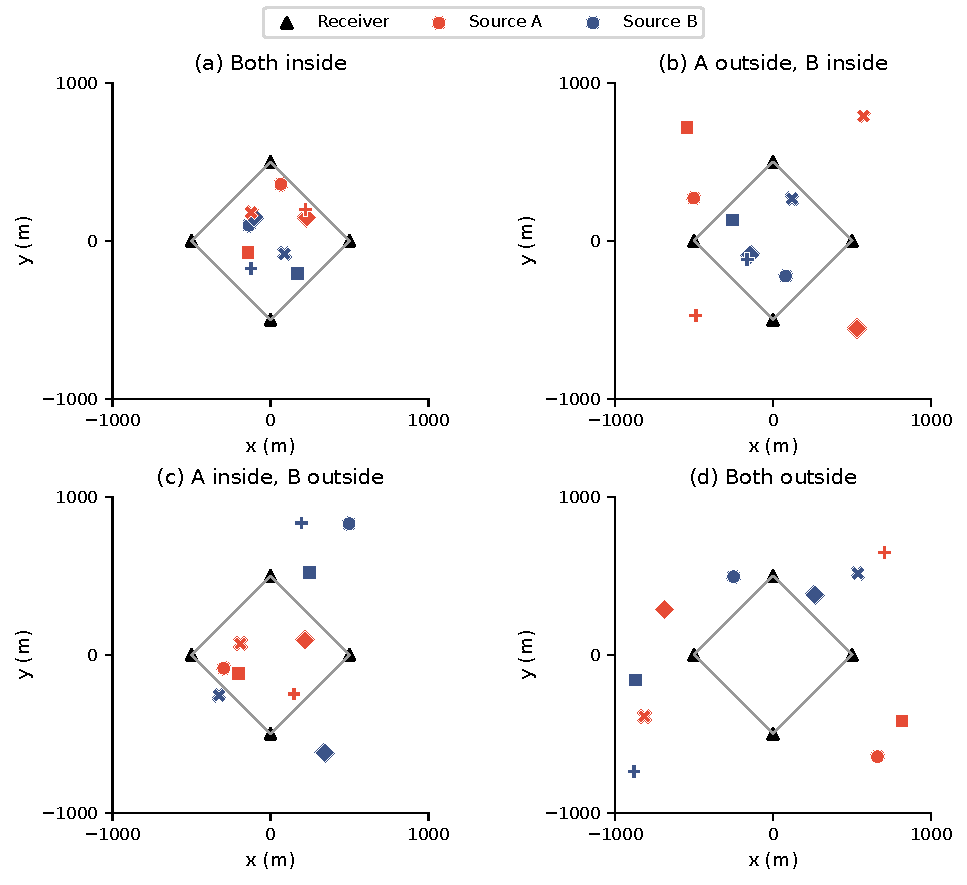
\includegraphics[width=.90\linewidth]{figures/formal_geometry.pdf}
\caption{20个源构型，每类5个。黑色三角形表示接收站；每个面板内，同形状配对源A（红）与源B（蓝），菱形为站点凸包。}\label{en:geometry}
\end{figure}

各方法使用相同IQ、传播信息、双精度计算和初始网格，保留各自初始化与连续精修。适配后的目标在下节说明。

AP分支在归一化目标上采用共同投影梯度阈值$10^{-8}$，关闭目标差停止项，局部迭代上限为100。VP-BNOMP及固定系数参照采用循环能量阈值$10^{-8}$，每次局部Newton最多五步，步长上限50\,m，小于0.01\,m的接受步触发局部退出，循环安全上限10000。梯度与能量条件不代表相同优化精度。完整方法比较使用冻结的原生规则，联合精修与曲率配对则明确匹配相应停止条件。

以$i$标记$n$条观测，每条先以平方距离作一次最优指派\cite{Kuhn1955}，所有位置指标共用这次匹配：
\begin{equation}
\pi^*=\arg\min_\pi\sum_k\|\widehat{\bm p}_{\pi(k)}-\bm p_k\|^2,
\quad e_{ik}=\|\widehat{\bm p}_{i,\pi^*(k)}-\bm p_{ik}\|.
\end{equation}
RMSE为$\sqrt{n^{-1}\sum_i e_{ik}^2}$，经验CDF为$n^{-1}\sum_i\mathbf1(e_{ik}\le t)$，均包含全部观测。双源成功要求$\max_k e_{ik}\le20$\,m，这是预设的$0.02R$误差门槛，与网格间隔区分。无效输出作为失败保留在分母中；本报告各批次均返回两个有限位置。

完整耗时包括DFT、选频、传输、搜索、系数估计、精修及必要输出检查，并同步GPU。若包含轨迹记录与末端诊断，其成本也计入；文件读取、磁盘写入及离线统计不计入，预热单列。加速比例使用同批结果。环境为Windows、Python 3.10.20、NumPy 2.2.6、PyTorch 2.8.0+cu129、RTX 4070 Ti SUPER和20个CPU线程，响应与目标采用双精度。重采样将同一实现的六档功率差作为一组。候选成本和曲率区间条件于固定布局，后文另行说明更广的分层区间。

\FloatBarrier
\subsection{基线目标与实现}
LS谱取峰连续精修式\eqref{en:single}的两个分离极大值，不作双源联合拟合。协方差方法将同一记录划分为$S$个不重叠片段，长度$N_s=N/S$；片段DFT $\bm z_{bf}\in\C^L$按$1/N_s$归一化，
\begin{equation}
\widehat{\bm C}_f=S^{-1}\sum_{b=1}^S\bm z_{bf}\bm z_{bf}^H.
\end{equation}
零均值模型下相关矩阵等于协方差矩阵。片段噪声方差为$\sigma_t^2/N_s$，仅保留相同物理处理频带，不跨随机实现拼接快拍。

MUSIC要求$K<L$、响应列线性独立、源协方差满秩及空间白噪声\cite{WeissAmar2005}。以$\bm E_{n,f}$收集最小$L-K$个特征值对应的特征向量，宽带评分与扣噪权重为
\begin{align}
S_{\rm MU}(\bm p)&=\left[\sum_f w_f\bm q_f^H
\bm E_{n,f}\bm E_{n,f}^H\bm q_f\right]^{-1},\\
\widetilde w_f&=\max\{\tr(\widehat{\bm C}_f)-L\sigma_t^2/N_s,0\},
\qquad w_f=\widetilde w_f/\sum_v\widetilde w_v.
\end{align}
权重之和为零时使用均匀权重。已知$K$确定子空间维度，有限样本精度仍取决于有效快拍和各频点信号功率。

MVDR在$\bm h_f^H\bm q_f=1$下最小化$\bm h_f^H\bm C_{f,\delta}\bm h_f$，其中$\bm h_f\in\C^L$为合成权重\cite{Capon1969}。对角加载与跨频平均给出
\begin{equation}
\begin{split}
\bm C_{f,\delta}&=\widehat{\bm C}_f+
\delta\,\tr(\widehat{\bm C}_f)\bm I_L/L,\\
S_{\rm MV}(\bm p)&=F_s^{-1}\sum_f
[\bm q_f^H\bm C_{f,\delta}^{-1}\bm q_f]^{-1}.
\end{split}
\end{equation}
无量纲加载$\delta$乘以平均对角功率。MVDR-known使用已知相对响应与上述频率平均，与DPD-HR原式区分\cite{TirerWeiss2016}。

SBL定义字典$\bm D_f=[\bm q_f(\bm g_1),\ldots,\bm q_f(\bm g_G)]$，逐频系数$\bm z_f\sim\mathcal{CN}(0,\bm\Gamma)$在频率间独立，共享非负功率$\bm\Gamma=\operatorname{diag}(\bm\gamma)$\cite{Nannuru2019}。协方差、后验均值、负对数证据与固定点更新为
\begin{align}
\bm C_f&=\sigma_f^2\bm I_L+\bm D_f\bm\Gamma\bm D_f^H,\qquad
\bm\mu_f=\bm\Gamma\bm D_f^H\bm C_f^{-1}\bm x_f,\\
\mathcal E(\bm\gamma)&=F^{-1}\sum_f
[\log\det\bm C_f+\bm x_f^H\bm C_f^{-1}\bm x_f],\\
\gamma_j^+&=\gamma_j\left[
\frac{\sum_f|\bm d_{fj}^H\bm C_f^{-1}\bm x_f|^2}
{\sum_f\bm d_{fj}^H\bm C_f^{-1}\bm d_{fj}}
\right]^{1/2},
\end{align}
其中$\bm d_{fj}$为$\bm D_f$的第$j$列，更新通过证据回溯控制。每五轮对八个活动位置作离网优化，每维位移不超过20\,m；L-BFGS-B坐标尺度为1000\,m，最多20轮。最终以单点$\gamma_j$选峰。每五轮检查停止：归一化证据变化低于$10^{-5}$、功率$\ell_1$相对变化低于1\%、输出与活动位置移动低于0.05\,m，连续两次满足后停止，最多300轮。

充分AP使用五个候选，反复条件搜索与位置精修，最多六个外层循环。多初值ML由四个唯一谱峰组合和四个Sobol空间初值最小化$J$，删除无序重复组合。GA-ML将四个坐标编码为个体，种群128、精英四个、锦标赛规模三，使用模拟二进制交叉（概率0.9、指数15）与多项式变异（每维概率0.25、指数20）\cite{DebAgrawal1995}；连续30代停滞或达到200代时停止，再联合精修最优个体。

固定系数BNOMP参照（FC--FC）由下式求导：
\begin{equation}
L_{\rm FC}(\bm p)=E_x^{-1}\sum_f
\|\bm y_f-\bm a_f(\bm p)q_f^{(0)}\|^2,
\label{en:fixedcoef}
\end{equation}
$q_f^{(0)}$在当前位置拟合，在求导及参照回溯中固定，接受后重新估计。多频块结构沿用\cite{Yang2022}，Hessian修正、边界和回溯为数值保护。两个标签依次表示曲率和试探接受目标。VP-BNOMP采用消元曲率与消元接受目标（VP--VP）。原始NOMP也将固定增益曲率与重估增益后的接受判断结合\cite{Mamandipoor2016}，因此另以固定系数曲率配合消元接受目标（FC--VP），隔离曲率变化的作用。

MUSIC使用四段；MVDR-known使用八段，$\delta=0.01$。AP局部调用最多25次线搜索、100轮迭代；交替精修最多12轮扫描，初始单源精修的相对容差为$10^{-12}$。BNOMP将Hessian特征值下限设为$10^{-9}$，在搜索边界内依次尝试$1,1/2,1/4,1/8,1/16$步长因子，其余上限及AP梯度阈值见前文。所有参数在比较前冻结。

\FloatBarrier
\subsection{共同观测比较与扩大验证}
表\ref{en:common}在同一240条观测上比较全部方法。MCJ-AP与充分AP、SBL均全部恢复，但完整成本明显较低。SBL的弱源误差分布更宽；两种BNOMP恢复相同228条，波形消元版平均成本较低。
\begin{table}[pos=H]\centering\small
\caption{共同240条观测。RMSE单位为m，耗时均值、中位数及P95单位为s；各指标保留全部观测。}\label{en:common}
\begin{tabular}{@{}lrrrrrr@{}}\toprule
方法 & 成功/240 & RMSE A & RMSE B & 均值 & 中位数 & P95\\\midrule
LS peaks & 38 & 191.982 & 845.184 & 0.2368 & 0.2181 & 0.3297\\
WB-MUSIC & 151 & 93.515 & 646.892 & 0.2015 & 0.1893 & 0.2719\\
MVDR-known & 75 & 320.684 & 804.082 & 0.1925 & 0.1807 & 0.2625\\
Full AP & 240 & 0.876 & 1.596 & 8.9076 & 9.1483 & 12.2348\\
BNOMP (FC--FC) & 228 & 0.906 & 89.706 & 2.9416 & 1.4625 & 8.1989\\
VP-BNOMP & 228 & 0.875 & 86.177 & 0.5907 & 0.3921 & 1.3971\\
Multistart ML & 45 & 256.061 & 776.935 & 1.2227 & 1.0868 & 2.5595\\
GA-ML & 185 & 279.056 & 501.231 & 8.0702 & 8.1102 & 9.0229\\
WB-SBL & 240 & 1.096 & 3.743 & 44.1296 & 36.8237 & 97.7075\\
MCJ-AP ($M=5$) & 240 & 0.876 & 1.596 & 0.7081 & 0.6347 & 1.0232\\\bottomrule
\end{tabular}\end{table}

\begin{figure}[pos=H]\centering
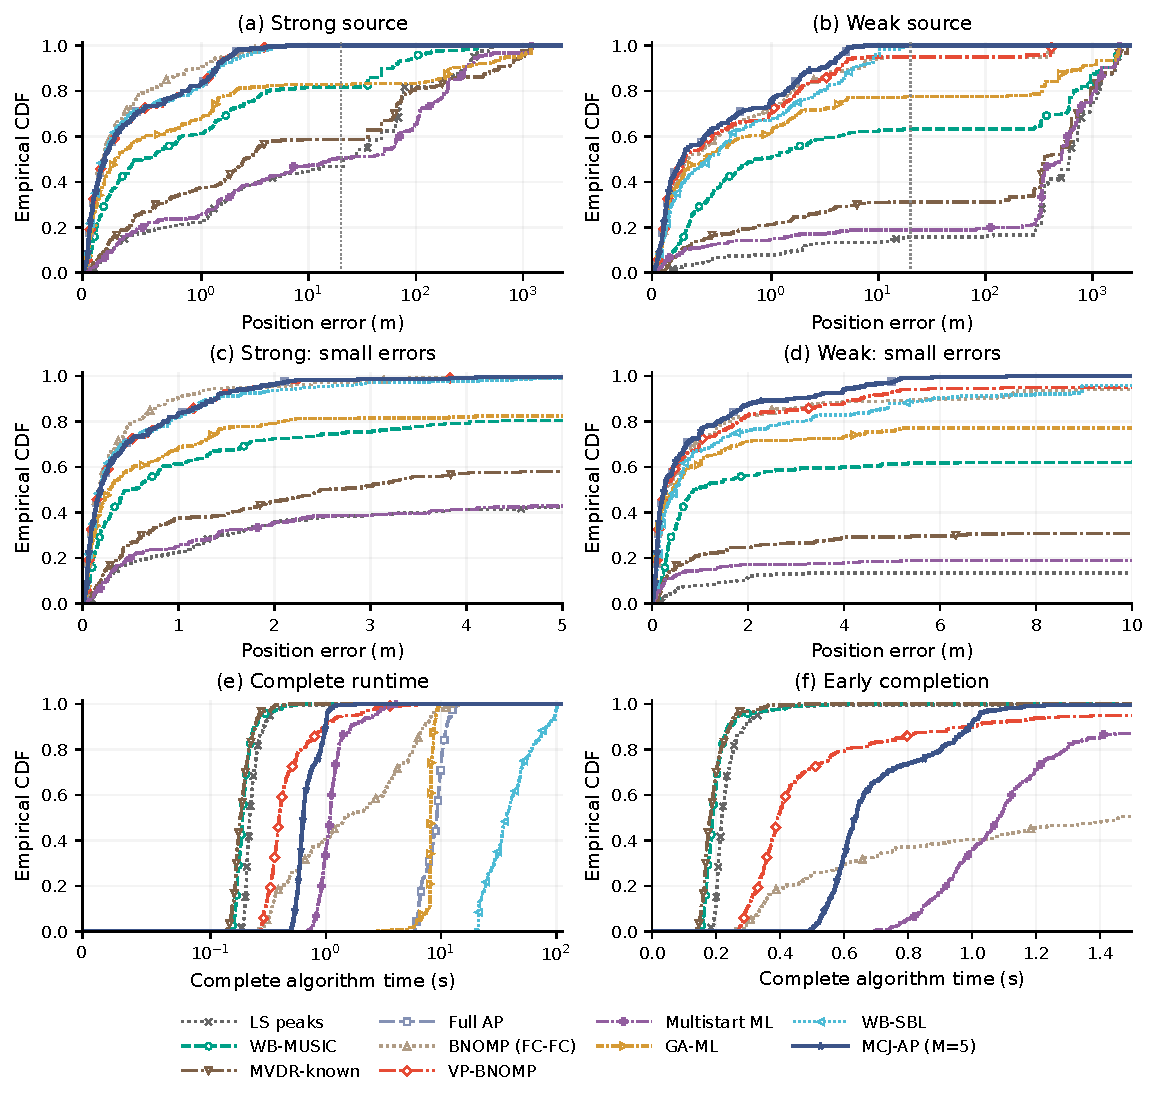
\includegraphics[width=\linewidth]{figures/assignment_cost_20261019/common_cdf.pdf}
\caption{共同240条的误差与完整耗时CDF。误差图包含全范围与小误差放大，耗时图包含全范围与早期完成情况。全范围坐标近零线性、超过阈值后对数，误差竖线为20\,m；曲线分母均包含全部观测。}\label{en:commoncdf}
\end{figure}
图\ref{en:commoncdf}区分典型精度与大误差尾部。AP误差曲线近乎重合；VP-BNOMP在多数观测中准确，但弱源仍有远距离错误，偶尔耗时较长。谱方法较快，其失败主要表现为大误差，而非轻微越过门槛。

\begin{figure}[pos=H]\centering
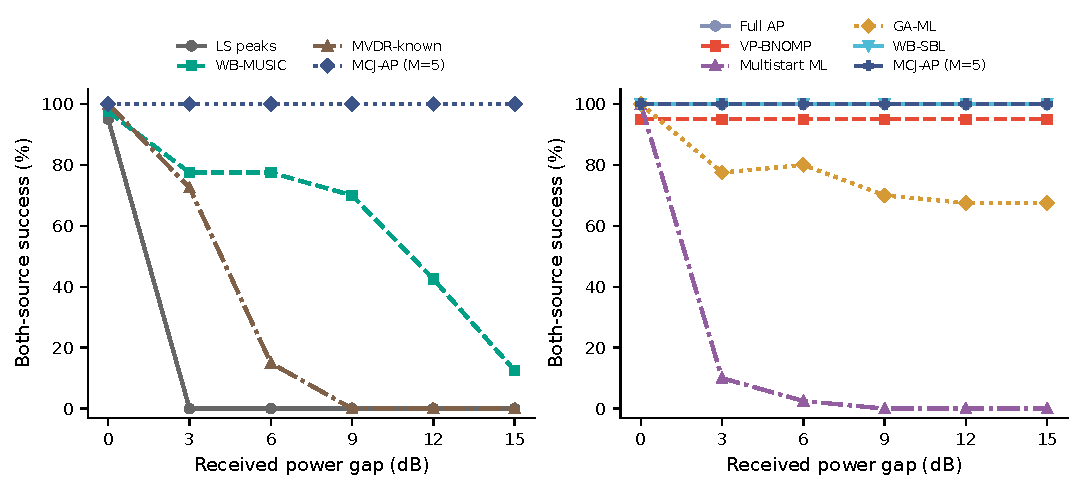
\includegraphics[width=\linewidth]{figures/formal_common.pdf}
\caption{共同子集的功率差扫描，每档40条观测。两个面板使用同一五候选AP参照。}\label{en:power}
\end{figure}
功率差增大时，MUSIC和MVDR-known的恢复能力下降（图\ref{en:power}）；第\ref{en:windowcheck}节检查有限窗失配能否解释所测失败。充分AP与多初值ML优化同一联合目标却得到不同结果，表明初始化与搜索影响明显。GA有208条、SBL有14条达到迭代上限，其余方法无触顶退出；全部输出均保留。

共同子集的保存输出中，五候选AP、充分AP与SBL分别在0.75、1.5和30\,s首次全部成功。这些检查点描述已记录结果，不构成可执行的提前停止规则。本批VP只记录最终完整输出，不同记录时序不足以支持严格的任意时刻性能排名。

\begin{table}[pos=H]\centering\small
\caption{2400条扩大验证。RMSE单位为m，完整耗时单位为s。VP-BNOMP耗时来自另一个同输入批次，受控加速比例使用配对批次计算。}\label{en:core}
\begin{tabular}{@{}lrrrrrr@{}}\toprule
方法 & 成功/2400 & RMSE A & RMSE B & 均值 & 中位数 & P95\\\midrule
AP ($M=1$) & 2280 & 0.897 & 107.265 & 0.3958 & 0.3700 & 0.5104\\
AP ($M=2$) & 2280 & 0.897 & 103.698 & 0.4704 & 0.4329 & 0.6340\\
MCJ-AP ($M=5$) & 2376 & 0.896 & 46.984 & 0.7180 & 0.6495 & 1.0267\\
VP-BNOMP & 2278 & 0.892 & 74.193 & 0.5855 & 0.3693 & 1.2470\\\bottomrule
\end{tabular}\end{table}
2400条观测中，五候选将AP成功率从95\%提高至99\%（表\ref{en:core}）。分层重采样所得成功率95\%区间为[96.83\%,100\%]；相对两候选增加四个百分点，其区间为[0,12.17]个百分点，反映了收益集中于一个构型。共同240条与扩大样本分开报告，不作为独立观测累加。

\begin{figure}[pos=H]\centering
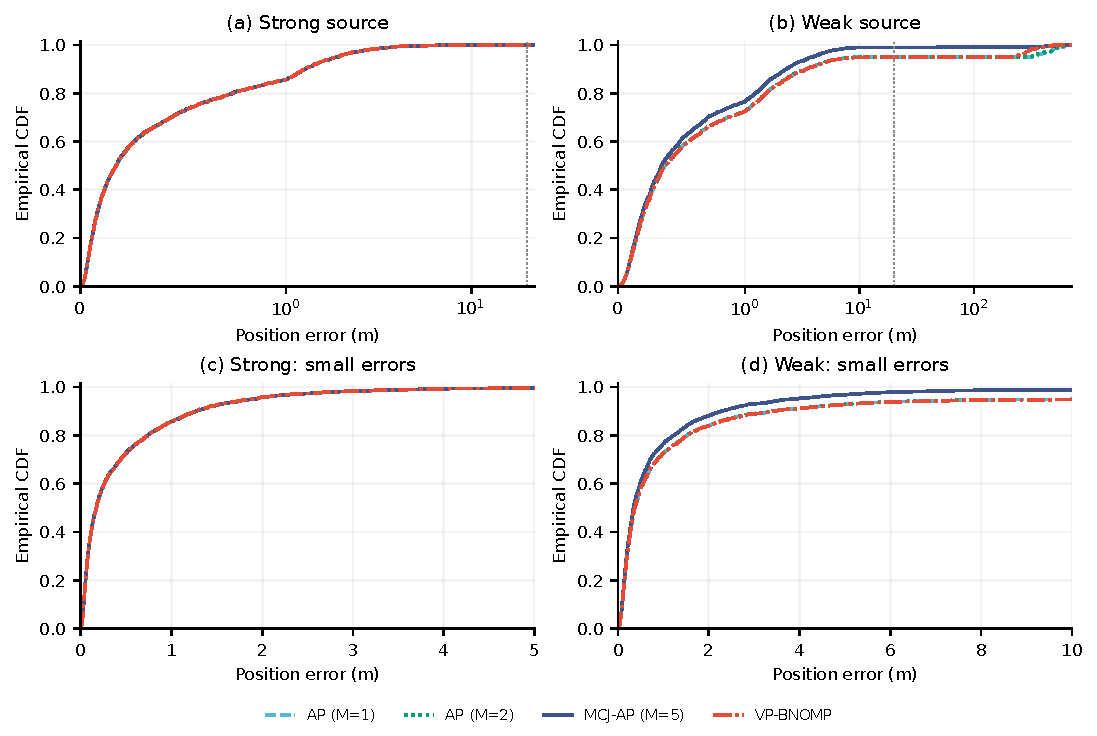
\includegraphics[width=\linewidth]{figures/assignment_cost_20261019/core_error_cdf.pdf}
\caption{全部2400条核心观测的强、弱源误差CDF。上排展示全范围，下排放大小误差；各曲线均包含失败观测。}\label{en:corecdf}
\end{figure}
强源CDF近乎重合（图\ref{en:corecdf}），弱源的小误差部分也相近，但尾部不同。五候选AP弱源P95为3.85\,m，RMSE为46.98\,m；构型4包含其全部24例失败，并贡献各档功率差下超过99.7\%的弱源平方误差。
\begin{figure}[pos=H]\centering
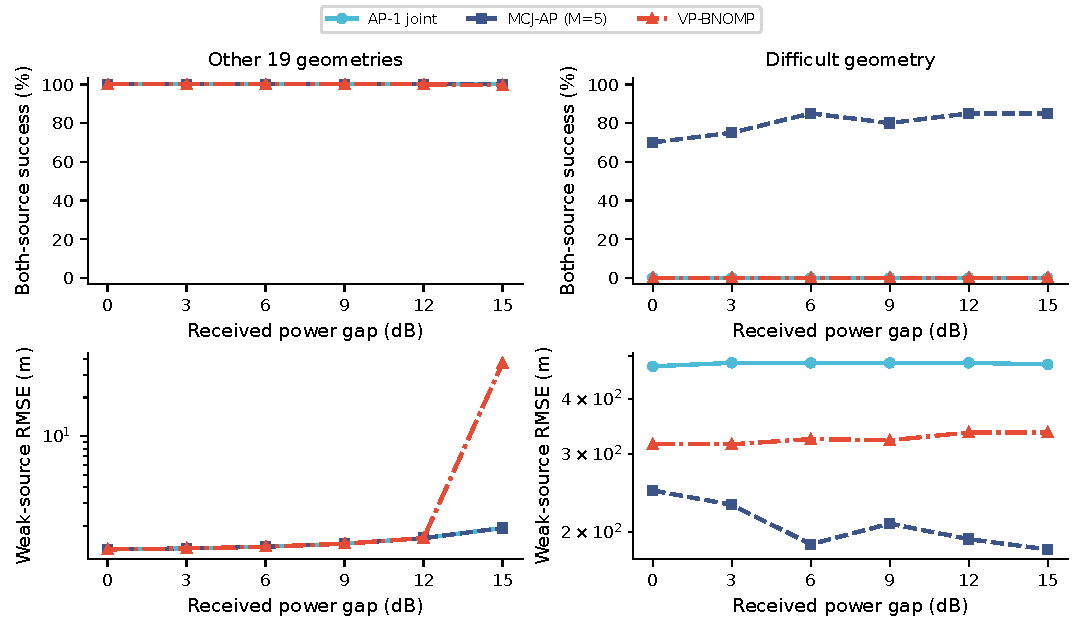
\includegraphics[width=.92\linewidth]{figures/formal_core.pdf}
\caption{其余19个构型（2280条）与构型4（120条）的功率差结果。这一诊断分组不从总体统计中删除任何观测。}\label{en:powergroups}
\end{figure}
其余构型中，AP弱源RMSE随功率差从1.31增至1.93\,m（图\ref{en:powergroups}）。VP在构型1的15\,dB下有两例失败，使这19个构型的RMSE为15.25\,m，AP约为1.52\,m。在构型4中，VP将弱源RMSE从单候选AP的479.66\,m降至325.07\,m，但仍未达到20\,m门槛。总体RMSE的非单调变化主要由构型4造成，各档功率差的几何不变。

\FloatBarrier
\subsection{候选覆盖与联合精修成本}\label{en:refinementcost}
AP新增的96例恢复均来自低排名条件候选。表\ref{en:candidaterank}按初始条件评分顺序，统计首个成功精修分支的排名。成功判定只在离线评价时使用真实位置，MCJ-AP仅依据最终残差$J$选取分支。恢复全部位于构型4，涉及20次波形／噪声实现中的18次；该构型另24条观测的五个精修分支均未成功。

\begin{table}[pos=H]\centering\small
\caption{全部2400条观测中，按初始条件评分排序的首个成功精修分支；两源匹配误差均不超过20\,m记为成功。}\label{en:candidaterank}
\begin{tabular}{@{}lrrrrrr@{}}\toprule
首个成功分支排名 & 1 & 2 & 3 & 4 & 5 & 无\\\midrule
观测数 & 2280 & 0 & 1 & 8 & 87 & 24\\\bottomrule
\end{tabular}\end{table}
96例恢复中，87例需要第五候选。存在成功分支的2376条观测均由最终残差选中了成功分支，其他观测没有损失原有成功。因此，在这一构型中，初始条件评分较低的候选仍可产生有效的连续定位解。

\begin{figure}[pos=H]\centering
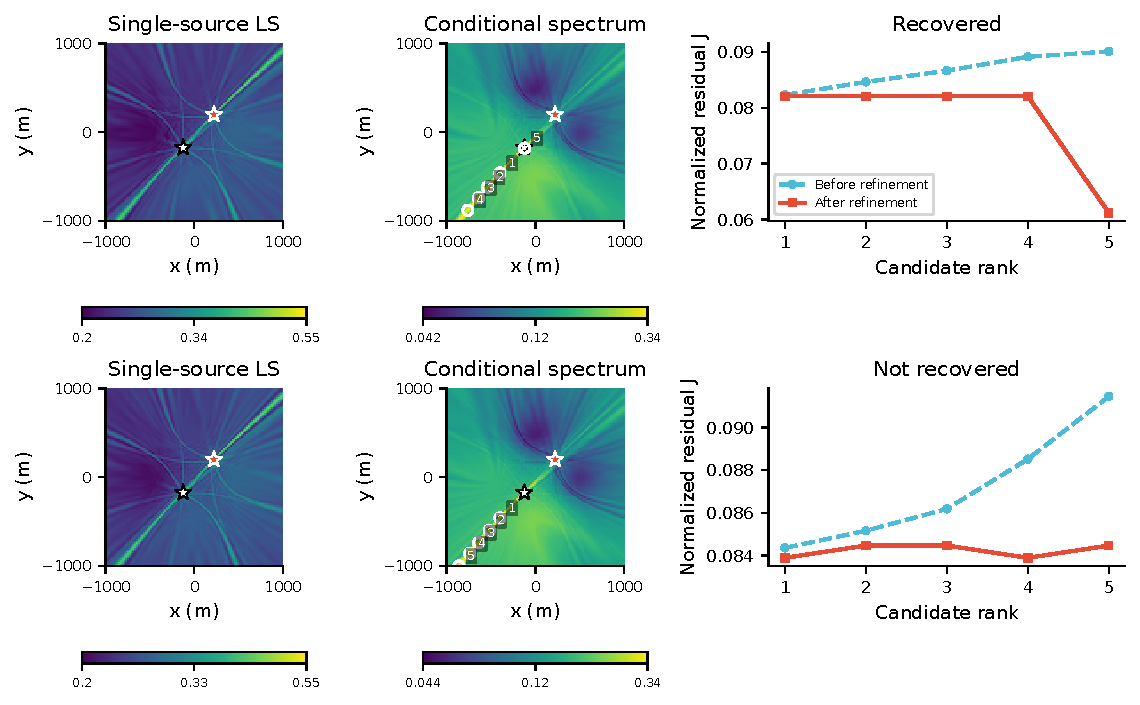
\includegraphics[width=\linewidth]{figures/formal_candidates.pdf}
\caption{构型4在0\,dB下的两个事后诊断案例。各列为单源谱、条件谱及精修前后分支残差。上例由第五候选恢复，下例没有有效候选；右图连线连接分支编号，并非优化轨迹。}\label{en:cases}
\end{figure}
图\ref{en:cases}上例的前四分支进入远端区域，第五分支获得更低的最终残差，弱源误差约0.09\,m。下例最近候选距源B仍约397\,m，精修未能恢复。两个案例分别展示了低排名分支恢复定位，以及五个局部精修分支均未成功的情况。

\begin{figure}[pos=H]\centering
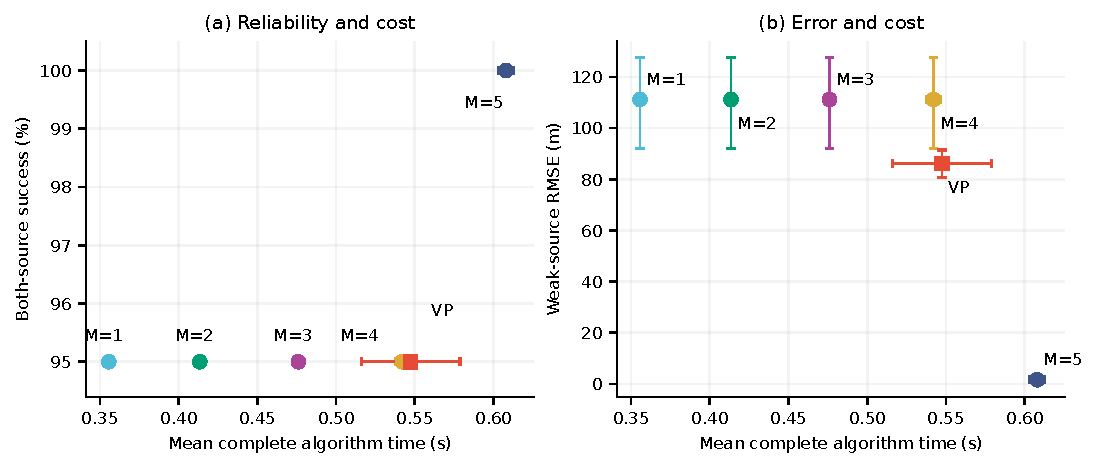
\includegraphics[width=\linewidth]{figures/assignment_cost_20261019/candidate_tradeoff.pdf}
\caption{AP的$M=1$--5与VP-BNOMP在同一240条观测上独立完整求解，并在同批交错计时。误差线为固定源位置构型内按实现配对重采样的95\%区间，保留六档功率差的关联。}\label{en:tradeoff}
\end{figure}
该批$M=1$--4均成功228条，平均耗时从0.3556增至0.5420\,s，弱源RMSE约111.2\,m。VP-BNOMP成功228条，弱源RMSE为86.18\,m，平均耗时0.5474\,s；五候选AP全部成功，平均0.6079\,s、弱源RMSE为1.60\,m。VP中位耗时0.3674\,s，单候选AP为0.3514\,s；VP耗时P95为1.3147\,s，五候选AP为0.7201\,s。双方均成功的228条中，VP在197条上比五候选AP快，后者恢复其余12条。这些结果区分了典型速度、恢复能力与耗时尾部。完整样本的保存分支前缀回放中，三、四候选分别成功2281、2289条，仅用于位置结果分析。

\begin{table}[pos=H]\centering\small
\caption{2400条观测上，对相同五候选作交替与联合精修。两种选中输出均满足同一投影梯度阈值。}\label{en:apjoint}
\begin{tabular}{@{}lrrrrr@{}}\toprule
精修 & 成功数 & RMSE B/m & 平均耗时/s & $J$调用 & 梯度调用\\\midrule
交替 & 2376 & 46.983 & 1.0840 & 204.21 & 198.21\\
联合 & 2376 & 46.984 & 0.7441 & 120.36 & 114.36\\\bottomrule
\end{tabular}\end{table}
处理相同五候选时，联合精修将成本降低31.36\%（表\ref{en:apjoint}）。两者使用同一完整投影目标及选中输出的投影梯度阈值，逐条成功／失败身份一致，强源RMSE均约0.896\,m，弱源P95均约3.85\,m。梯度调用减少42.30\%，与优化调用减少相符，而非停止规则放宽。联合减交替耗时的配对分层95\%区间为$[-0.3691,-0.3121]$\,s。每个构型的平均成本均降低，节省11.42\%--48.04\%。两个未选中的交替分支达到局部上限，仍计入成本。这一节省针对固定候选数下的精修；增加候选的恢复与额外成本另由图\ref{en:tradeoff}评价。

\FloatBarrier
\subsection{隔离波形消元曲率的作用}
表\ref{en:common}的固定系数／VP对照同时改变局部曲率与接受目标，平均耗时减少79.92\%。为隔离曲率，另一配对批次统一以$\phi_j$接受试探。FC--VP使用$H_{zz}$求方向，VP--VP使用$H_{\rm VP}$；两者采用相同的源发现和初始化流程、条件系数与梯度计算公式、数值保护、消元目标回溯及循环能量停止准则。受控改动仅为局部曲率构造，实际位置与残差轨迹可以不同。
\begin{table}[pos=H]\centering\small
\caption{相同波形消元接受目标下的曲率比较，共240条配对观测；更新与循环数为每条均值。}\label{en:curvaturetable}
\begin{tabular}{@{}lrrrrrr@{}}\toprule
版本 & 成功数 & RMSE A/m & RMSE B/m & 平均耗时/s & 更新数 & 循环数\\\midrule
FC--VP & 228/240 & 0.906 & 89.706 & 5.574 & 1498.82 & 810.90\\
VP--VP & 228/240 & 0.875 & 86.177 & 0.905 & 135.55 & 47.97\\\bottomrule
\end{tabular}\end{table}
两者成功／失败身份相同，均按原生能量规则停止。平均完整耗时下降83.77\%，固定布局配对95\%区间为[81.73\%,85.58\%]；中位数由2.836降至0.567\,s，P95由16.161降至2.538\,s。VP--VP在240条中的170条更快，平均节省尤其来自较慢案例的改善。更新与循环次数的下降支持式\eqref{en:rate}的曲率机制。

两版本平均核心耗时为5.5483、0.8987\,s，记录与最终检查另计0.0254、0.0059\,s。480组历史／当前VP配对的输入、位置、目标、计数、停止原因及保存路径一致，但绝对墙钟不同。因此各加速比例使用本批配对：79.92\%对应整个局部更新变化，83.77\%对应同接受目标下的曲率变化。后者区间采用布局内4000次配对bootstrap（种子20261020），保留每次实现的六档功率差。相同能量阈值并未要求最终联合梯度满足共同容差，第\ref{en:localchecks}节进一步检查这一差别。

终态质量统一用完整联合目标$J$及其箱约束投影梯度的无穷范数评价，坐标单位为m。以$10^{-10}$为目标差绝对容差，VP--VP在199组中取得更低的$J$，41组近似相等，没有更高的情况；容差改为$10^{-8}$时分别为167、73和零组。目标差绝对值的中位数为$3.34\times10^{-7}$，P95为$7.37\times10^{-6}$，最大差$1.97\times10^{-3}$出现在两种方法均定位失败的观测中。VP--VP在全部240组中具有更小的投影梯度范数，其中位数为$1.30\times10^{-7}$，FC--VP为$2.03\times10^{-6}$。因此，在原生停止规则下，计算节省未伴随这些终态拟合与驻点指标恶化；定位质量仍由位置误差评价。

\FloatBarrier
\subsection{新源位置上的冻结方法验证}
表\ref{en:new}与图\ref{en:newcdf}评价16个新构型。两种AP均恢复全部480条，误差近乎相同，五候选成本约为单候选的1.96倍。首分支已经有效，新增分支没有增加成功数。结合构型4可见，固定候选预算保留了首候选无效时的恢复机会，但首分支已经有效时不会主动减少计算。
\begin{table}[pos=H]\centering\small
\caption{新源构型480条观测，接收站位置不变。RMSE单位为m，完整耗时单位为s。}\label{en:new}
\begin{tabular}{@{}lrrrrrr@{}}\toprule
方法 & 成功/480 & RMSE A & RMSE B & 均值 & 中位数 & P95\\\midrule
AP ($M=1$) & 480 & 0.958 & 2.194 & 0.461 & 0.456 & 0.545\\
MCJ-AP ($M=5$) & 480 & 0.958 & 2.194 & 0.906 & 0.893 & 1.078\\
VP-BNOMP & 390 & 202.882 & 206.261 & 1.051 & 0.629 & 4.245\\\bottomrule
\end{tabular}\end{table}
\begin{figure}[pos=H]\centering
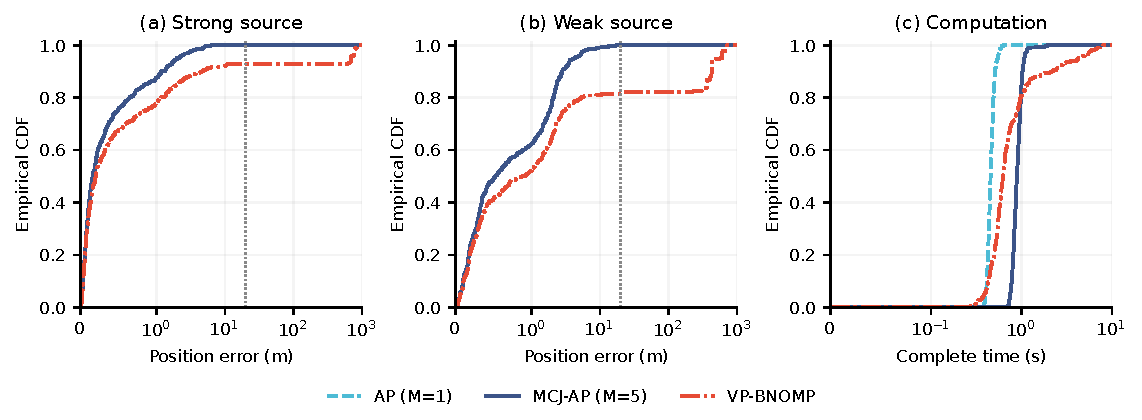
\includegraphics[width=\linewidth]{figures/review_supplement_20261020/independent_cdf.pdf}
\caption{新480条观测的误差与完整耗时CDF。AP误差曲线近乎重合；保留全部观测，误差参考线为20\,m。全范围坐标近零线性，超过标注阈值后为对数。}\label{en:newcdf}
\end{figure}
VP-BNOMP的90例失败分布于新构型8、9、14、15，分别为30、25、30、5例。每档功率差15例，其中55例仅B失败、33例双源失败、两例仅A失败，涉及全部五次随机实现。失败样本平均耗时1.448\,s，成功样本为0.959\,s；失败样本均按能量稳定停止，最终目标高于AP。它们从首个保存完整位置对起就失败，后续也未成功，因而不能归因于丢弃已保存的成功解或安全上限截断。记录从一次双源循环后开始，无法进一步区分最初的发现错误与某一步更新错误。

\FloatBarrier
\subsection{有限窗与数值核验}
\label{en:windowcheck}
八条开发观测（四类构型，各取0、15\,dB）提供保存的无噪声分量。在真实位置处，定义有限窗残差和预计投影后噪声能量
\begin{equation}
E_{\rm win}=\sum_{b,f}\|\bm\Pi_{\bm A_f}^{\perp}\bm z_{bf}^{(0)}\|^2,
\qquad E_n=SF_s(L-K)\sigma_t^2/N_s.
\end{equation}
所有$\bm A_f$均满列秩。一、四、八段时，残差占比分别为0.209--0.382\%、0.756--1.387\%、1.529--2.854\%；相应$E_{\rm win}/E_n$为0.035--0.882、0.126--3.210、0.238--6.611。较短窗口增加模型失配。

在同观测上比较矩形窗、周期Hann窗及4096点Hann长窗的四个重叠帧。窗化噪声方差为$\sigma_t^2\sum_n w[n]^2/N_s^2$，重叠帧不视为独立快拍。15\,dB下，长窗将$E_{\rm win}/E_n$降至0.076--0.294，但MUSIC与MVDR-known仍仅恢复1/4、0/4，失败身份不变；0\,dB时均为4/4。将干净源分量投影到真实响应后再恢复原噪声，可消除几乎全部模型残差，但七个失败方法--观测对仍无恢复。该真值辅助诊断不参加排名，说明有限窗失配不足以解释所测失败。

\label{en:localchecks}
数值收敛与定位误差分别检查。在八条开发观测上，将原生VP路径继续迭代至联合投影梯度达到$10^{-8}$，成功数仍为8/8，弱源RMSE从3.22变为3.25\,m，含梯度检查的平均完整耗时由0.382增至0.860\,s。

另以八条开发观测检查FC--FC小步机制，与正式FC--VP／VP--VP配对区分。循环能量容差取$10^{-8}$、$10^{-7}$、$10^{-6}$时，成功数为8/8、7/8、6/8，平均耗时为5.478、2.318、0.971\,s，导数调用为2679.5、1133.9、467.4。仅取消小步局部退出，得到8/8、8.011\,s和4758.4次调用；$10^{-8}$下的波形消元得到8/8、0.436\,s和70.4次调用。参照的21436次更新全部接受，83.67\%短于0.01\,m，没有Hessian修正、步长裁剪、回溯缩步或边界裁剪。两个站外源诊断位置的原始步长经消元从0.0138／0.0111\,m增至11.25／32.26\,m，实际仍需回溯接受。四个保存位置的解析消元Hessian与自动微分的最大绝对差约$1.4\times10^{-18}$。这些检查为正式曲率配对提供机制依据，完整成本仍以配对测量为准。

\FloatBarrier
\section{总结}
本文针对两个未知宽带重叠源的直接定位，研究候选选择和局部更新成本。MCJ-AP保留条件谱峰，直到两源位置完成联合精修后再择优。保存分支说明了初始评分为何可能舍弃有效解：所测困难构型中的大多数额外恢复需要第五候选。联合L-BFGS-B则在共同投影梯度停止容差下减少处理同一批候选的成本。VP-BNOMP将波形消元纳入局部位置曲率，相同接受目标下的配对证实其平均成本和更新次数下降，所测终态残差与投影梯度范数未变差。新源构型测试区分了这些收益与完整流程的可靠性：额外AP候选在该批没有增加恢复，VP仍有失败。在本文同步、已知响应的基带模型下，证据支持延后分支选择的候选恢复作用，以及消元曲率的局部计算效率收益。后续可研究候选预算分配与未知源数。

% Before submission, confirm funding, competing interests and data/code availability.
% No such declarations are inferred from the research results.
\FloatBarrier
\appendix
\FloatBarrier
\section{新源位置坐标}\label{en:coordinates}
表\ref{en:coordinates-table}列出新源坐标，单位为m，保留六位小数。类别1--4依次表示双源均在接收站凸包内、A外B内、A内B外、双源均在外。几何与波形种子为20261020071、20261020072，随机实现编号1000--1004，构型按一基编号。新位置满足与原样本相同的几何排除条件，不依据方法成绩筛选。
\begin{table}[pos=H]\centering
\caption{新源位置。仅缩放A，B与噪声固定。}\label{en:coordinates-table}
\begin{tabular}{@{}rrrrrr@{}}\toprule
编号 & 类别 & $x_A$ & $y_A$ & $x_B$ & $y_B$\\\midrule
1 & 1 & -209.742960 & -211.672998 & -135.426339 & 121.578497\\
2 & 1 & -115.361316 & 76.809910 & 67.769590 & -192.728293\\
3 & 1 & -208.559801 & 115.499630 & 268.616751 & -92.726639\\
4 & 1 & 173.459164 & -110.441904 & -168.154517 & -145.923194\\
5 & 2 & -926.529606 & 771.380729 & -198.481435 & 152.456653\\
6 & 2 & -628.314566 & -929.843027 & -55.519139 & -297.939120\\
7 & 2 & -195.757938 & -496.419920 & 157.528284 & 224.885259\\
8 & 2 & -734.894082 & -306.033731 & -249.535479 & 71.485648\\
9 & 3 & -64.564529 & 351.783227 & 663.100329 & 428.023655\\
10 & 3 & -166.451414 & 260.105867 & 823.995321 & 431.176047\\
11 & 3 & 74.808116 & 299.580428 & -702.622192 & 474.464614\\
12 & 3 & -162.472651 & -112.907043 & 765.537745 & -808.531366\\
13 & 4 & 313.792247 & 602.900501 & 700.222844 & -274.728424\\
14 & 4 & 482.010461 & 239.752856 & 888.180085 & 90.857032\\
15 & 4 & -374.838719 & 599.269525 & 240.800462 & 663.866438\\
16 & 4 & 624.598019 & 542.011213 & -163.287363 & 904.989973\\\bottomrule
\end{tabular}\end{table}
\FloatBarrier
\bibliographystyle{\PaperRoot template/cas-model2-names}
\bibliography{\PaperRoot references/references}
\end{document}
